% !TEX root = main.tex

%------------------------------------------------
%\newpage
\chapter[Cauchy's Integral Formula]{Cauchy's Integral Formula and its Applications}
\section{Cauchy's Integral Formula}
We have seen so far that if $f:\mathcal{R} \to \C$ is holomorphic on a starlit region $\mathcal{R}$ then
\[
\int_{\mathcal{C}} f = 0
\]
for any closed contour $\mathcal{C}$ in $\mathcal{R}$. What happens when $\mathcal{R}$ is not starlit?  

It may happen that while $\mathcal{R}$ itself is not starlit, the contour $\mathcal{C}$ is contained in a starlit subregion $\mathcal{S}$ of $\mathcal{R}$.

\begin{figure}[h]
\makebox[\linewidth][c]{
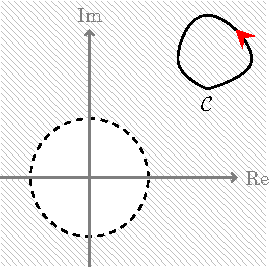
\includegraphics[scale=1]{notsc3}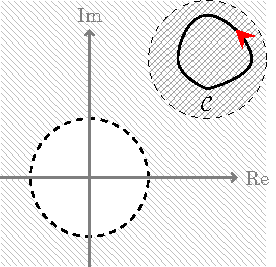
\includegraphics[scale=1]{notsc1}\quad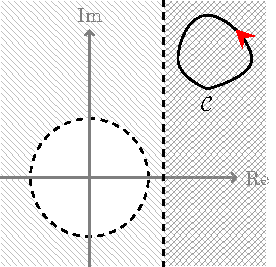
\includegraphics[scale=1]{notsc2}
}
\caption{The region $\mathcal{R}$ consists of the complex plane with a disc centred at the origin removed.  This region is not starlit, but there are starlit subregions of $\mathcal{R}$ containing the contour $\mathcal{C}$.}
\end{figure}

Thus if $f$ is holomorphic on $\mathcal{R}$, then $f$ is also holomorphic on $\mathcal{S}$ and so Cauchy's Theorem for Starlit Regions (Theorem~\ref{t:cauchyst}) gives
\[
\int_{\mathcal{C}} f=0.
\]


If $\mathcal{R}$ is not simply connected, then it may not be possible to do this; in particular, when $\mathcal{C}$ encloses a point $z_0$ at which $f$ is not holomorphic.  For example, suppose $f:\C \backslash \set{0} \to \C$ is defined by $f(z) = \dfrac{1}{z}$, and $\mathcal{C}$ is the contour shown in Figure~\ref{f:notsc}.  
\begin{figure}[h]
\centering
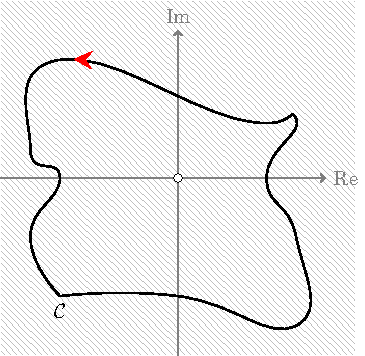
\includegraphics[scale=0.75]{notsc}
\caption{A contour $\mathcal{C}$ contained in the non-simply connected region $\C\backslash \set{0}$.}
\label{f:notsc}
\end{figure}

Here $\C \backslash \set{0}$ is not starlit, and there is no starlit subregion of $\C \backslash \set{0}$ containing $\mathcal{C}$.  Nonetheless, in certain circumstances, it is at least possible to replace $\mathcal{C}$ something easier in order to calculate the integral.

\begin{definition}
A contour $\mathcal{C}$, that is not closed, is said to be \emph{simple} if $\mathcal{C}$ does not intersect itself.  A \emph{simple closed contour $\mathcal{C}$} is one that does not intersect itself except that its start point is the same as its end point.
\end{definition}

\begin{figure}[h]
\centering
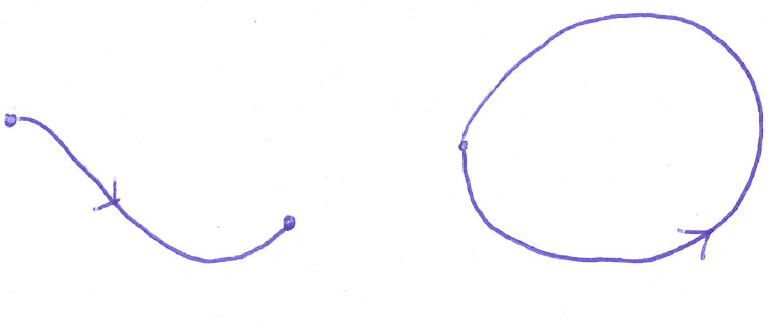
\includegraphics[scale=0.3]{simple_full}
\caption{Simple contours.}
\end{figure}
\begin{figure}[h]
\centering
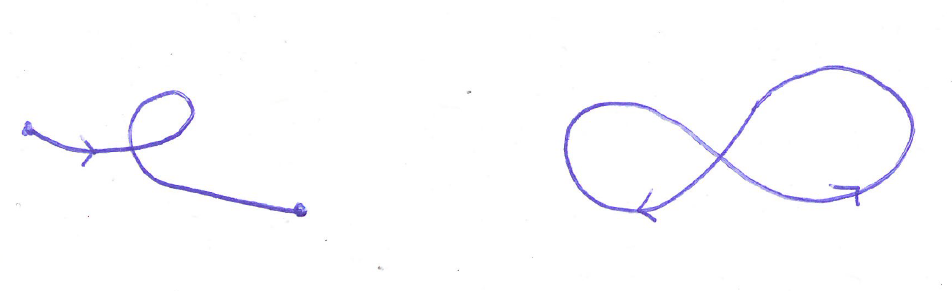
\includegraphics[scale=0.3]{nonsimple_full}
\caption{Non-simple contours.  Note that the closed, non-simple contour on the right has no obvious orientation - it is neither clockwise nor anticlockwise.}
\end{figure}


For a simple closed contour $\mathcal{C}$, when we speak of $\mathcal{C}$ being clockwise or anticlockwise, we mean relative to the points enclosed by $\mathcal{C}$.  In other words, a contour $\mathcal{C}$ is anticlockwise if, as we travel along $\mathcal{C}$, the region enclosed by $\mathcal{C}$ always lies to our left.  Again, we shall avoid giving a precise definition, and treat this notion informally.



%\begin{comment}
%Of course, even when $\mathcal{R}$ is simply connected, it will not always be true that $\mathcal{C}$ is contained in a starlit subregion of $\mathcal{R}$; for example, consider the contour $\mathcal{C}$ shown in Figure~\ref{f:scnotstarlit1}.
%\begin{figure}[h]
%\centering
%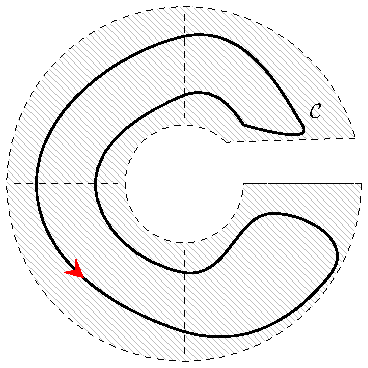
\includegraphics[scale=1]{scnotstarlit2}
%\caption{A contour $\mathcal{C}$ contained in a simply connected region that is not starlit.}
%\label{f:scnotstarlit1}
%\end{figure}
%
%\vspace*{10cm}
%\end{comment}



The following Theorem shows us how in some cases, a potentially complicated contour integral may be reduced to an easier one.
\begin{theorem}[Shrinking Contour Theorem/Deformation Theorem]
\label{t:sc}
Let $\mathcal{R}$ be a simply connected region, $\mathcal{C}$ an anticlockwise, simple closed contour in $\mathcal{R}$, $z_0$ a point enclosed by $\mathcal{C}$ and $g$ a function which is holomorphic on $\mathcal{R} \backslash \set{z_0}$.  Then
\[
\int_{\mathcal{C}} g = \int_{\mathcal{C}_r} g
\]
where $\mathcal{C}_r$ is an anticlockwise circular contour with centre $z_0$ and radius $r$, which is small enough so that $\mathcal{C}_r$ is contained in $\mathcal{R}$.
\end{theorem}

\begin{center}
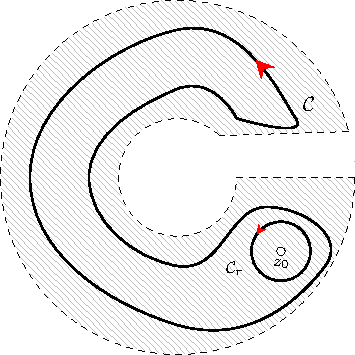
\includegraphics[scale=0.75]{scnotstarlit4}
\end{center}

\begin{proof}\emph{(This is an informal sketch of the proof)}

Since $\mathcal{R}$ is simply connected,  we can partition $\mathcal{R}$ into starlit subregions $\mathcal{R}_1,\mathcal{R}_2,\ldots, \mathcal{R}_n$, numbered so that $z_0 \in \mathcal{R}_n$. By joining points on $\mathcal{C}$, we get anticlockwise closed contours $\mathcal{C}^{(1)},\mathcal{C}^{(2)},\ldots,\mathcal{C}^{(n)}$, with $\mathcal{C}^{(j)}$ contained in $\mathcal{R}_j$ for each $j$.  Label the regions $\mathcal{R}_j$ so that $z_0 \in \mathcal{R}_n$. 

%\begin{figure}[h]
%\centering
%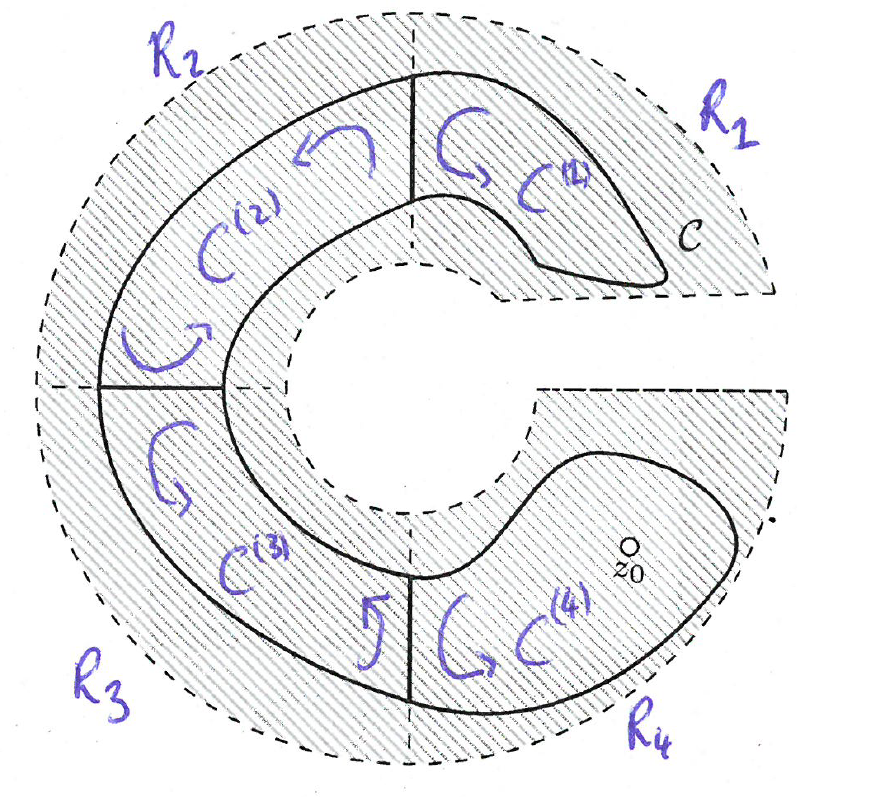
\includegraphics[scale=0.3]{deformation1_full}
%\end{figure}

%\vspace*{12cm}
Note that
\[
\int_{\mathcal{C}} g = \int_{\mathcal{C}^{(1)}} g + \int_{\mathcal{C}^{(2)}} g + \ldots + \int_{\mathcal{C}^{(n)}} g,
\]
as the integrals along the connecting edges cancel in pairs.

% Sorry, you can't have floats within the proof environment (not in outer par mode!) [DE 14.07.17]
%\begin{figure}[h]
%\centering
\begin{center}
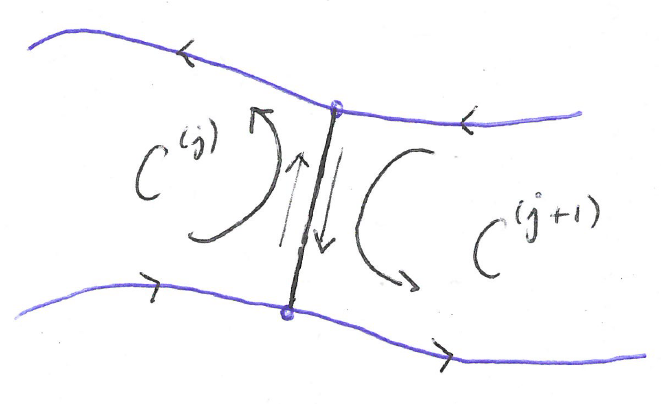
\includegraphics[scale=0.3]{deformation2_full}
\captionof{figure}{The edge where $\mathcal{C}^{(j)}$ and $\mathcal{C}^{(j+1)}$ intersect is traversed in one direction along $\mathcal{C}^{(j)}$ and in the opposite direction along $\mathcal{C}^{(j+1)}$.  Thus when we compute the sum of the integral of $g$ along $\mathcal{C}^{(j)}$ and along $\mathcal{C}^{(j+1)}$, the contributions made by this connecting edge cancel.}
\end{center}
%\end{figure}

Moreover, for each $j \neq n$, $g$ is holomorphic on $\mathcal{R}_j$, and $\mathcal{C}^{(j)}$ is a closed contour contained in the starlit region $\mathcal{R}_j$.  Thus by Cauchy's Theorem for Starlit regions, we have
\[
\int_{\mathcal{C}^{(j)}} g = 0\quad \text{ for } j=1,2,\ldots,n-1.
\]
Combining these two observations it follows that
\[
\int_{\mathcal{C}} g = \int_{\mathcal{C}^{(n)}} g,
\]
and thus we need to show that
\[
\int_{\mathcal{C}^{(n)}}g = \int_{\mathcal{C}_r} g.
\]

%XXX

\begin{absolutelynopagebreak}
While $\mathcal{R}_n$ is starlit, $\mathcal{R}_n \backslash \set{z_0}$ is not.  Thus we split $\mathcal{R}_n \backslash \set{z_0}$ into two starlit subregions, and construct contours $S_1$ and $S_2$ by connecting $\mathcal{C}^{(n)}$ and $\mathcal{C}_r$ as shown.
\begin{center}
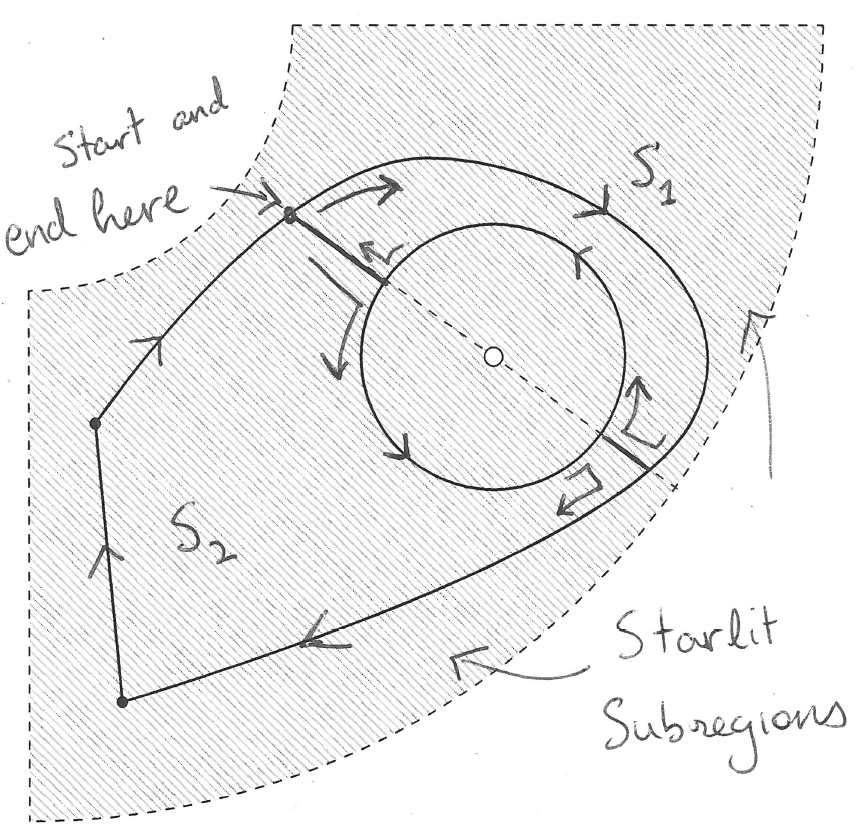
\includegraphics[scale=0.25]{shrinking}
\end{center}
\end{absolutelynopagebreak}

By Cauchy's Theorem for Starlit Regions, we again have
\[
\int_{S_1} g = \int_{S_2} g = 0.
\]

Notice that if we join $S_1$ and $S_2$ we get a contour consisting of
\begin{itemize}
\item An anticlockwise copy of the circular contour $\mathcal{C}_r$, 
\item A clockwise copy of $\mathcal{C}^{(n)}$, i.e. the reverse of $\mathcal{C}^{(n)}$, and
\item two copies of each of the new edges connecting $\mathcal{C}^{(n)}$ and $\mathcal{C}_r$, one in each direction.
\end{itemize}
Thus we get
\[
\int_{S_1} g + \int_{S_2} g = \int_{\mathcal{C}_r} g - \int_{\mathcal{C}^{(n)}} g
\]
as the integrals along the new edges connecting $\mathcal{C}^{(n)}$ and $\mathcal{C}_r$ cancel, and we are left with $\mathcal{C}_r$ and the reverse of $\mathcal{C}^{(n)}$.
  
Hence
\[
0 = \int_{S_1} g + \int_{S_2} g = \int_{\mathcal{C}_r} g - \int_{\mathcal{C}^{(n)}} g
\]
and so
\[
\int_{\mathcal{C}_r} g = \int_{\mathcal{C}^{(n)}} g = \int_{\mathcal{C}} g.
\]

%\vspace*{9cm}

\end{proof}

\endinput

A very similar argument is used to prove Cauchy's Theorem for Simply Connected Regions (which we stated previously as Theorem~\ref{t:cauchysc}).

\begin{theorem}[Cauchy's Theorem for Simply Connected Regions]
Let $f$ be a function that is holomorphic in a simply connected region $\mathcal{R}$, and let $\mathcal{C}$ be a closed contour in $\mathcal{R}$. Then
\[
\int_{\mathcal{C}} f = 0.
\]
\end{theorem}
\begin{proof}
This is identical to the Proof of Theorem~\ref{t:sc}, except that now, $f$ is holomorphic on the starlit region $\mathcal{R}_n$, so that
\[
\int_{\mathcal{C}} f = \int_{\mathcal{C}_r} f =0.
\]
\end{proof}


%\vspace*{7cm}

%XXXXX



\begin{theorem}[Cauchy's Integral Formula]
\label{t:cauchyformula}
Let $\mathcal{R}$ be a simply connected region, $\mathcal{C}$ an anticlockwise simple closed contour in $\mathcal{R}$, $z_0$ a point enclosed by $\mathcal{C}$ and $f$ a function that is holomorphic on $\mathcal{R}$.  Then
\[
\int_{\mathcal{C}} \frac{f(z)}{z-z_0} \ dz = 2 \pi i f( z_0).
\]
\end{theorem}
\begin{proof}
Define a new function $g$ by the formula
\[
g(z) = \frac{f(z)}{z-z_0}
\]
so that $g$ is holomorphic on $\mathcal{R} \backslash \set{z_0}$, i.e., where $f$ is holomorphic and $z-z_0 \neq 0$.  Thus we are trying to show that
\[
\int_{\mathcal{C}} g = 2\pi i f(z_0).
\]
Using the Shrinking Contour Theorem~\ref{t:sc}, we may replace $\mathcal{C}$ with an anticlockwise circular contour $\mathcal{C}_r$ with centre $z_0$ and radius $r$ to get
\[
\int_{\mathcal{C}} g = \int_{\mathcal{C}_r} g
\]
whenever $r>0$ is small enough so that $\mathcal{C}_r$ is contained in $\mathcal{R}$.  

If we define $I$ by
\[
I = \left(\int_{\mathcal{C}_r} \frac{f(z)}{z-z_0}\ dz \right) - 2 \pi i f(z_0),
\]
then we want to show that $I=0$.  To do this, we will write $I$ as a single integral along $\mathcal{C}_r$ and use the Estimation Lemma (together with the fact that our definition of $I$ does not depend on our choice of sufficiently small $r$).

We know from a question on Exercise Sheet 2 that
\[
\int_{\mathcal{C}_r} \frac{1}{z-z_0}\ dz = 2\pi i,
\]
and therefore, since $f(z_0)$ is a constant, we get
\[
2\pi i f(z_0) = \int_{\mathcal{C}_r} \frac{f(z_0)}{z-z_0}\ dz.
\]
Thus
\begin{align*}
I &= \int_{\mathcal{C}_r} \frac{f(z)}{z-z_0}\ dz - \int_{\mathcal{C}_r} \frac{f(z_0)}{z-z_0}\ dz \\
& = \int_{\mathcal{C}_r} \frac{f(z)-f(z_0)}{z-z_0}\ dz.
\end{align*}
To apply the Estimation Lemma, we need to find an upper bound for
\[
\abs{ \frac{f(z)-f(z_0)}{z-z_0} } \quad \text{ where } z \in \mathcal{C}_r.
\]
Since $\mathcal{C}_r$ is a circle with centre $z_0$ and radius $r$, it is clear that $\abs{z-z_0} = r$ for all $z \in \mathcal{C}_r$, and thus we look at $\abs{f(z)-f(z_0)}$.

Since $f$ is holomorphic on $\mathcal{R}$, it is continuous on $\mathcal{R}$ and in particular, continuous at $z_0$.  Thus given any $\epsilon>0$ there exists $\delta>0$ such that
\[
0 < \abs{z-z_0} < \delta \Rightarrow \abs{ f(z)-f(z_0) } < \epsilon.
\]
In other words, given any $\epsilon >0$, if we choose $r$ so that $0<r < \delta$, we have
\[
z \in \mathcal{C}_r \Rightarrow \abs{z-z_0} = r < \delta \Rightarrow \abs{f(z)-f(z_0)} < \epsilon.
\]
For any such $r$ we thus have
\[
z \in \mathcal{C}_r \Rightarrow \abs{\frac{f(z)-f(z_0)}{z-z_0}} = \frac{\abs{f(z)-f(z_0)}}{\abs{z-z_0}} < \frac{\epsilon}{r}.
\]
By the Estimation Lemma (using the fact that $\ell ( \mathcal{C}_r ) = 2 \pi r$), we see that
\[
\abs{\int_{\mathcal{C}_r} \frac{f(z)-f(z_0)}{z-z_0}\ dz} \leq \frac{\epsilon}{r} 2 \pi r = 2\pi \epsilon.
\]
However, since the definition of $I$ does not depend on our choice of (small) $r$, it follows that
\[
\abs{I} < 2 \pi \epsilon
\]
for all $\epsilon>0$.  Hence $\abs{I}=0$ which implies $I=0$, or in other words,
\[
\int_{\mathcal{C}} \frac{f(z)}{z-z_0}\ dz = 2 \pi i f(z_0).
\]


\end{proof}

\begin{note}
Cauchy's Integral Formula, and its proof, can be easily remembered using the following approximation: if $r$ is small and $z \in \mathcal{C}_r$ then $f(z) \approx f(z_0)$, hence
\[
\int_{\mathcal{C}_r} \frac{f(z)}{z-z_0}\ dz \approx \int_{\mathcal{C}_r} \frac{f(z_0)}{z-z_0}\ dz = f(z_0) \int_{\mathcal{C}_r} \frac{1}{z-z_0}\ dz = f(z_0) (2\pi i).
\]
\end{note}
By Theorem~\ref{t:cauchyformula}, if the values of $f(z)$ are known for all $z$ along a closed contour $ \mathcal{C}$, then for any $z_0$ enclosed by $\mathcal{C}$, $f(z_0)$ may be calculated via
\[
f(z_0)= \frac{1}{2\pi i} \int_{\mathcal{C}} \frac{f(z)}{z-z_0}\ dz.
\]
Moreover, suppose we wish to evaluate the integral $\int_{\mathcal{C}} g$ of a continuous function $g$ along some closed contour $\mathcal{C}$.  If we can find some point $z_0$ enclosed by $\mathcal{C}$ and a function $f$ holomorphic on $\mathcal{R}$ with 
\[
g(z) = \frac{f(z)}{z-z_0} \quad \text{ for all }z \in \mathcal{C}
\]
then our integral may be evaluated using
\[
\int_{\mathcal{C}} g = \int_{\mathcal{C}} \frac{f(z)}{z-z_0}\ dz =  2\pi i f(z_0).
\]
In other words, it is enough to know the value of $f(z_0)$ in order to calculate $\int_{\mathcal{C}}g$.
\begin{example}
Evaluate the integral
\[
\int_{\mathcal{C}} \frac{\Log (z)}{z^2+9}
\]
where $\Log$ is the Principal Logarithm function and $\mathcal{C}$ is the anticlockwise circle with centre $4i$ and radius $3$.
\end{example}
%\vspace*{5cm}
We know that $\Log$ is holomorphic on $\C_{\pi}$, and moreover, we have
\[
z^2+9 = (z+3i)(z-3i).
\]
If we write
\[
\frac{\Log (z)}{z^2+9} = \frac{\Log (z)}{(z+3i)(z-3i)} = \frac{f(z)}{z-z_0}
\]
where $z_0=3i$ and
\[
f(z) = \frac{\Log (z)}{z+3i}
\]
then $z_0$ is enclosed by $\mathcal{C}$ and $f$ is holomorphic on $\C_{\pi} \backslash \set{-3i}$, which is a region containing $\mathcal{C}$.
\begin{figure}[h]
\centering
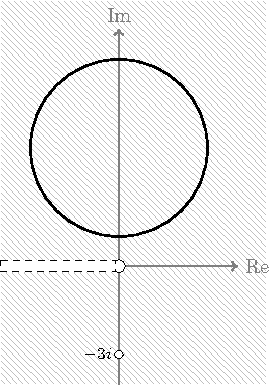
\includegraphics[scale=1]{cpi4}
\end{figure}
However, it is clear that the region $\C_{\pi} \backslash \set{-3i}$ is not simply connected, so the hypotheses of Cauchy's Integral Formula are not fully satisfied.  We deal with this by replacing $\C_{\pi} \backslash \set{-3i}$ with a subregion that is simply connected.

Indeed, if we consider the region $\mathcal{R} = \set{ z \in \C: \Im (z)>0}$, then we see that
\begin{itemize}
\item $\mathcal{R}$ is simply connected,
\item $f$ is holomorphic on $\mathcal{R}$, and
\item $\mathcal{C}$ is a simple, closed anticlockwise contour that is contained in $\mathcal{R}$ and encloses the point $z_0=3i$.
\end{itemize}
\begin{figure}[h]
\centering
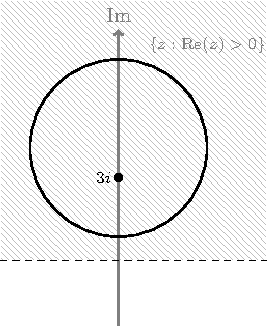
\includegraphics[scale=1]{cpi5}
\caption{The region $\mathcal{R}$ contains $\C_{\pi} \backslash \set{-3i}$ (there are many possible choices for $\mathcal{R}$).}
\end{figure}
Therefore, we can apply Cauchy's Integral Formula, which gives
\begin{align*}
\int_{\mathcal{C}} \frac{\Log(z)}{z^2+9}\ dz &= \int_{\mathcal{C}} \frac{f(z)}{z-z_0}\ dz \\
& = 2 \pi i f(z_0) \\
& = 2 \pi i \left( \frac{\Log(3i)}{3i+3i} \right) \\
& = \frac{\pi}{6} \left( \log (3) + i \frac{\pi}{2} \right).
\end{align*}

%\vspace*{5cm}



%\vspace*{8cm}

\begin{theorem}[Cauchy's Integral Formula for Derivatives]
\label{t:cauchyd}
Let $\mathcal{R}$ be a simply connected region, $\mathcal{C}$ a simple, closed anticlockwise contour contained in $\mathcal{R}$ and $f$ a function that is holomorphic on $\mathcal{R}$. Then
\begin{enumerate}
\item $f$ is infinitely differentiable on $\mathcal{R}$, and
\item At every point $z$ in the region enclosed by $\mathcal{C}$, the $k^{th}$ derivative $f^{(k)}$ of $f$ satisfies
\[
f^{(k)}(z) = \frac{k!}{2\pi i} \int_{\mathcal{C}} \frac{f(\zeta)}{(\zeta-z)^{k+1}}\ d \zeta.
\]
\end{enumerate}
\end{theorem}
\begin{proof} \emph{(Sketch)}
By Cauchy's Integral Formula, we have
\[
f(z) = \frac{1}{2\pi i} \int_{\mathcal{C}} \frac{f(\zeta)}{\zeta-z}\ d\zeta
\]
for any $z$ in the region enclosed by $\mathcal{C}$.  Hence
\[
f'(z) = \frac{d}{dz} \left[ \frac{1}{2\pi i} \int_{\mathcal{C}} \frac{f(\zeta)}{\zeta-z}\ d\zeta \right].
\] 
A somewhat technical argument shows that we may `differentiate under the integral sign' to get
\begin{align*}
f'(z) &= \frac{1}{2\pi i}\int_{\mathcal{C}} \frac{d}{dz} \left[ \frac{f(\zeta)}{\zeta-z} \right]\ d\zeta \\
& = \frac{1}{2\pi i} \int_{\mathcal{C}} -  \frac{f(\zeta)}{(\zeta-z)^2} (-1)\ d \zeta \\
& = \frac{1!}{2\pi i} \int_{\mathcal{C}}   \frac{f(\zeta)}{(\zeta-z)^2} \ d \zeta 
\end{align*}
(here we are using the fact that for $\zeta \in \mathcal{C}$, $\zeta-z \neq 0$ and so $z \mapsto \frac{f(\zeta)}{\zeta-z}$ is differentiable on the region enclosed by $\mathcal{C}$). Differentiating a second time gives
\begin{align*}
f''(z) &= \frac{1}{2\pi i} \int_{\mathcal{C}} (-2) \frac{f(\zeta )}{(\zeta-z)^3} (-2)\ d\zeta \\
& = \frac{2!}{2\pi i} \int_{\mathcal{C}} \frac{f( \zeta)}{(\zeta-z)^3}\ d\zeta.
\end{align*}
Continuing in this way we get the required expression for $f^{(k)}(z)$.
\end{proof}
\begin{theorem}[Liouville's Theorem]
Let $f:\C \to \C$ be holomorphic (i.e. $f$ is holomorphic on the entire complex plane) and suppose that $f$ is bounded, i.e., there exists $M>0$ with $\abs{f(z)}\leq M$ for all $z \in \C$.  Then $f$ is constant.
\end{theorem}
\begin{proof}
Exercise Sheet 4.
\end{proof}
\section{Evaluating Real Integrals Using Cauchy's Integral Formula}
An important application of Cauchy's Integral Formula (Theorem~\ref{t:cauchyformula}) is that it allows us to evaluate certain \emph{real} integrals that would be difficult, if not impossible, to evaluate otherwise.  The following example illustrates the general method for doing so, which we shall develop in the next few sections.
\begin{example}
\label{e:realint1}
Let us use contour integration to evaluate the real integral
\[
\int_{-\infty}^{+\infty} \frac{1}{1+x^2}\ dx.
\]
\end{example}
In order to apply Cauchy's Integral Formula, we need to choose an appropriate
\begin{itemize}
\item[(i)] contour $\mathcal{C}$ and
\item[(ii)] complex function $f$.
\end{itemize}
For the above integral, we will look at the function
\[
f:\C \backslash \set{ i,-i} \to \C, \quad f(z) = \frac{1}{1+z^2}
\]
which is holomorphic on $\C \backslash \set{i,-i}$, and the contour $\mathcal{C}_R = L_R + S_R$, where $L_R$ is the line segment $[-R,R]$, and $S_R$ is the semicircle with centre $0$, radius $R$, from $R$ through $iR$ to $-R$, where $R>1$.
\begin{center}
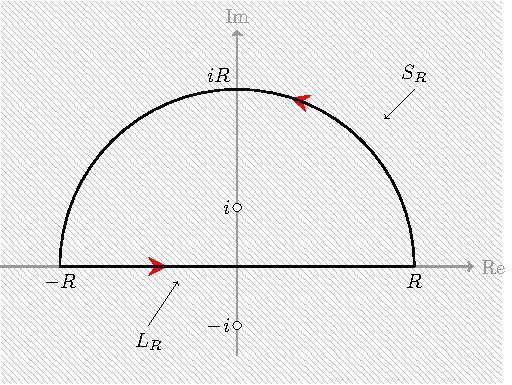
\includegraphics[scale=1]{semicircle8}
\end{center}
%\vspace*{8cm}
Write
\[
\frac{1}{1+z^2} = \frac{1}{(z+i)(z-i)} = \frac{g(z)}{z-z_0}
\]
where
\[
g(z) = \frac{1}{z+i}\quad \text{ and } z_0=i.
\]
Then $g$ is holomorphic on $\C \backslash \set{-i}$ and in particular, on the simply connected region $\mathcal{R} = \set{ z \in \C: \Im (z) > - \frac{1}{2}}$.  Moreover, $\mathcal{C}_R$ is a closed, simple anticlockwise contour in $\mathcal{R}$ and $z_0=i$ is a point enclosed by $\mathcal{C}_R$.
\begin{center}
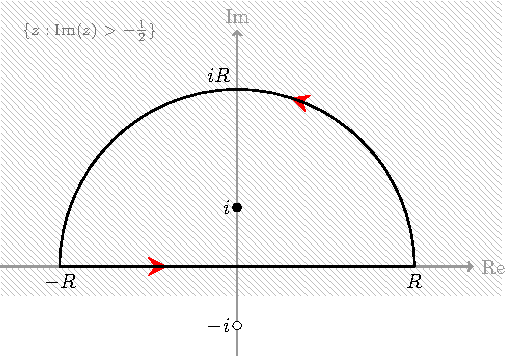
\includegraphics[scale=1]{semicircle9}
\end{center}
Hence by Cauchy's Integral Formula,
\begin{align*}
\int_{\mathcal{C}_R} \frac{1}{1+z^2}\ dz &= \int_{\mathcal{C}_R} \frac{g(z)}{z-i}\ dz \\
&= 2 \pi i g(i) \\
& = 2\pi i \frac{1}{i+i} = \pi.
\end{align*}
(Note that  this integral does not depend on the value of $R$ once $R>1$).
%\vspace*{5cm}


Having evaluated the integral using Cauchy's Integral Formula, we now look at the integrals along the two paths $L_R$ and $S_R$;
\[
\int_{\mathcal{C}_R} \frac{1}{z^2+1}\ dz = \int_{L_R} \frac{1}{z^2+1}\ dz + \int_{S_R} \frac{1}{z^2+1}\ dz.
\]
Parameterise $L_R$ with $\gamma_L:[-R,R] \to \C$, $\gamma(t)=t$, so that $\gamma'(t)=1$ and
\[
\int_{L_R} \frac{1}{1+z^2}\ dz = \int_{-R}^R \frac{1}{1+t^2}\ dt.
\]
We have seen already (Example~\ref{e:estimation}) that
\[
\lim_{R \to \infty} \int_{S_R} \frac{1}{1+z^2}\ dz = 0.
\]
Hence
\begin{align*}
\pi & = \lim_{R \to \infty} \int_{\mathcal{C}_R} \frac{1}{1+z^2}\ dz \\
& = \left( \lim_{R \to \infty} \int_{L_R} \frac{1}{1+z^2}\ dz \right) +  \left( \lim_{R \to \infty} \int_{S_R} \frac{1}{1+z^2}\ dz \right)  \\
& = \lim_{R \to \infty} \int_{-R}^R \frac{1}{1+t^2}\ dt + 0 \\
& = \int_{-\infty}^{\infty} \frac{1}{1+t^2}\ dt.
\end{align*}
So we have used contour integration to show that
\[
\int_{-\infty}^{\infty} \frac{1}{1+x^2}\ dx = \pi.
\]
%\vspace{15cm}

%\vspace*{5cm}

\begin{example}
\label{e:trig1}
Now let us consider the integral
\[
\int_{\mathcal{C}} \frac{-i}{6z^2+13z+6}\ dz
\]
where $\mathcal{C}$ is the anticlockwise contour whose points lie on the circle $\set{z \in \C: \abs{z}=1 }$. 
\end{example}
 We can evaluate this integral in two ways:
\begin{enumerate}
\item[(i)] Describe the contour by $\gamma:[0,2\pi] \to \C$, $\gamma(t) = \exp(it)$ (which is of course the same as $\gamma(t)=\cos (t) + i \sin (t)$).

Then $\gamma'(t)=ie^{it}$, and for all $z \in \mathcal{C}$
\begin{align*}
6z^2+13z+6 & = 6 \left[ e^{it} \right]^2 + 13 \left[ e^{it} \right] + 6 \\
& = 6 e^{2it} + 13 e^{it} + 6.
\end{align*}
Writing
\[
f(z) =  \frac{-i}{6z^2+13z+6}
\]
we have
\begin{align*}
f \left( \gamma(t) \right) \gamma ' (t) & = \frac{-i}{6e^{2it}+13e^{it}+6} \cdot ie^{it} \\
& = \frac{1}{6e^{it}+13+6e^{-it}} \\
& = \frac{1}{13+6[e^{it}+e^{-it}]}.
\end{align*}
But the since $\cos(t) = (e^{it}+e^{-it})/2$ we have
\[
6[e^{it}+e^{-it}] = 12 \cos (t),
\]
hence
\[
f \left( \gamma(t) \right) \gamma ' (t) = \frac{1}{13+12\cos (t)}.
\]
It follows that
\[
\int_{\mathcal{C}} \frac{-i}{6z^2+13z+6}\ dz=  \int_0^{2\pi} \frac{1}{13+12 \cos (t)}\ dt.
\]
However, we do not know how to evaluate the integral on the right.




\item[(ii)] Evaluate the integral using Cauchy's Integral Formula.  To do this we need to find
\begin{itemize}
\item A simply connected region $\mathcal{R}$ containing our contour $\mathcal{C}$,
\item A point $z_0$ enclosed by $\mathcal{C}$, and 
\item A function $g$ that is holomorphic on $\mathcal{R}$.
\end{itemize}
Then Cauchy's Integral formula will give
\[
\int_{\mathcal{C}} \frac{g(z)}{(z-z_0)}\ dz = 2 \pi i g(z_0).
\]
Of course, we want to choose $z_0$ and $g$ so that
\[
\frac{-i}{6z^2+13z+6} = \frac{g(z)}{z-z_0}.
\]
We have
\[
6z^2+13z+6 = (2z+3)(3z+2) = 6(z+\tfrac{3}{2})(z+\tfrac{2}{3}),
\]
which has zeros at $z=-\frac{3}{2}$ and $z= - \frac{2}{3}$.  It follows that $f$ is holomorphic on $\C \backslash \set{ - \frac{3}{2},- \frac{2}{3}}$.  Only the point $z_0=-\frac{2}{3}$ is enclosed by $\mathcal{C}$, so we let
\[
g(z)=  \frac{-i}{6(z+\frac{3}{2})},
\]
and note that
\[
f(z) = \frac{g(z)}{z-z_0}.
\]
The function $g$ is holomorphic on $\C \backslash \set{- \frac{3}{2}}$, and in particular, on the simply connected region $\mathcal{R} = \set{ z \in \C: \Re (z) > - \frac{5}{4}}$.
%\vspace*{9cm}
\begin{center}
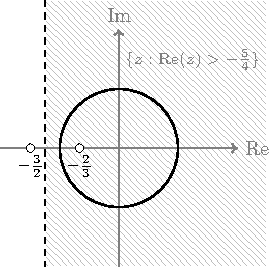
\includegraphics[scale=1]{righthalf}
\end{center}
Now, $\mathcal{C}$ is contained in $\mathcal{R}$ and encloses $z_0=-\frac{2}{3}$, and $g$ is holomorphic on $\mathcal{R}$, so that we may apply the integral formula to get
\begin{align*}
\int_{\mathcal{C}} \frac{-i}{6z^2+13z+6}\ dz & = \int_{\mathcal{C}} \frac{g(z)}{z-(-\frac{2}{3})}\ dz \\
& = 2\pi i g (-\tfrac{2}{3}) \\
& = 2\pi i \left( \frac{-i}{6(-\frac{2}{3}+\frac{3}{2})} \right) \\
& = \frac{2\pi }{5}.
\end{align*}
%\vspace*{10cm}
\end{enumerate}
Because methods (i) and (ii) must give the same value, we conclude that
\[
\int_0^{2\pi} \frac{1}{13+12\cos(t)}\ dt = \frac{2\pi}{5}.
\]



We can generalise the method of Example~\ref{e:trig1} to evaluate other real trigonometric integrals.
\begin{definition}
A \emph{Rational Function} $R:U \to \R$, where $U \subseteq \R^2$, is a function of the form
\[
R(x,y) = \frac{f(x,y)}{g(x,y)},
\]
where $f,g: \mathbb{R}^2 \to \R$ are two polynomials in $x$ and $y$ with real coefficients.
\end{definition}
We will now describe how to use contour integration to evaluate integrals of the form
\[
\int_0^{2\pi} R( \cos (t), \sin (t) )\ dt,
\]
where $R$ is a rational function of two real variables.  Note that $\cos$ and $\sin$ are periodic with period $2\pi$, and that the above integral has limits $0$ and $2\pi$.




For example, if $R$ is defined by
\[
R(x,y) = \frac{1}{16x^2+25y^2},
\]
then we are looking at the integral
\[
\int_0^{2\pi} R(\cos (t) , \sin (t) )\ dt = \int_0^{2\pi} \frac{1}{16 \left( \cos (t) \right)^2+25 \left( \sin (t) \right)^2}\ dt.
\]
 We want to rewrite this as the contour integral of a complex function $f$.


  In order to do this we will choose
\begin{enumerate}
\item[(i)] a suitable complex function $f$,
\item[(ii)] a suitable contour $\mathcal{C}$, and
\item[(iii)] a suitable parameterisation $\gamma: [a,b] \to \C$ of $\mathcal{C}$ so that
\[
\int_{\mathcal{C}} f = \int_a^b f \left( \gamma (t) \right) \gamma' (t)\ dt = \int_0^{2\pi} R( \cos (t) , \sin (t))\ dt.
\]
\end{enumerate}
For $\mathcal{C}$, we use the unit circle, parameterised by $\gamma:[0,2\pi] \to \C,\ \gamma(t) = \exp(it)$.  We want to choose $f$ so that
\[
f( \gamma(t)) \gamma'(t) = R( \cos(t),\sin(t) ) \quad \text{ for } t \in [0,2\pi].
\]
 For $z \in \mathcal{C}$, $z= \exp(it)$ for some $t \in [0,2\pi]$ and so
\begin{align*}
\cos(t) & = \frac{\exp(it)+\exp(-it)}{2}  = \frac{z+z^{-1}}{2} \\
\sin(t) & = \frac{\exp(it)-\exp(-it)}{2i} =  \frac{z-z^{-1}}{2i} \\
\gamma'(t) & = i \exp(it) = iz.
\mbox{ hence }
 R ( \cos (t), \sin (t) )  &= R \left( \frac{z+z^{-1}}{2}, \frac{z-z^{-1}}{2i} \right).
\end{align*}
Thus if we define $f$ by 
\[
f(z) = R \left( \tfrac{1}{2}(z+z^{-1}),\tfrac{1}{2i}(z-z^{-1}) \right) \cdot \frac{1}{iz}
\]
we have
\begin{align*}
f( \gamma(t)) \gamma'(t) & = R \left( \tfrac{1}{2}(z+z^{-1}),\tfrac{1}{2i}(z-z^{-1}) \right) \cdot \frac{1}{iz} \cdot iz \\
&= R( \cos(t),\sin(t) ) 
\end{align*}
whenever $z = \gamma(t) \in \mathcal{C}$.
Thus
\[
\int_{\mathcal{C}} f = \int_0^{2\pi} R \left( \cos(t) , \sin (t) \right)\ dt.
\]
\begin{example}
Use contour integration to evaluate
\[
\int_0^{2\pi} \frac{1}{5-3\cos (t)}\ dt.
\]

If we denote the integrand by $R(\cos(t),\sin(t))$, we let
\begin{align*}
f(z) &= R \left[ (z+z^{-1})/2 , (z-z^{-1})/(2i) \right] \cdot \frac{1}{iz}\\
& = \frac{1}{5-3[z+z^{-1}]/2} \cdot \frac{1}{iz} \\
& = \frac{-2i}{10z-3z^2-3} \\
& = \frac{2i}{3z^2-10z+3} \\
& = \frac{2i}{(3z-1)(z-3)}.
\end{align*}
It follows that
\[
\int_0^{2\pi} \frac{1}{5-3\cos (t)}\ dt = \int_{\mathcal{C}} \frac{2i}{(3z-1)(z-3)}\ dz
\]
where $\mathcal{C}$ is the anticlockwise circle $\abs{z}=1$.

The point $z_0=\frac{1}{3}$ is the only point enclosed by $\mathcal{C}$ at which $f$ is not holomorphic.  If we let
\[
g(z) = \frac{2i}{3(z-3)}
\]
we have
\[
\frac{g(z)}{z-\frac{1}{3}} = \frac{2i}{(3z-1)(z-3)}
\]
and $g$ is holomorphic on the simply connected region $\set{z \in \C: \Re (z) < 2}$, which contains $\mathcal{C}$.  Hence
\begin{align*}
\int_0^{2\pi} \frac{1}{5-3 \cos(t)}\ dt &= \int_{\mathcal{C}} \frac{2i}{(3z-1)(z-3)}\ dz \\
& = \int_{\mathcal{C}} \frac{g(z)}{z-\frac{1}{3}}\ dz \\
& = 2\pi i g(\tfrac{1}{3}) \\
& = 2\pi i \left( - \frac{i}{4} \right) = \frac{\pi}{2}.
\end{align*}


\end{example}


